\chapter{Code}
\label{sec:a-kapitel}


\label{motorH}
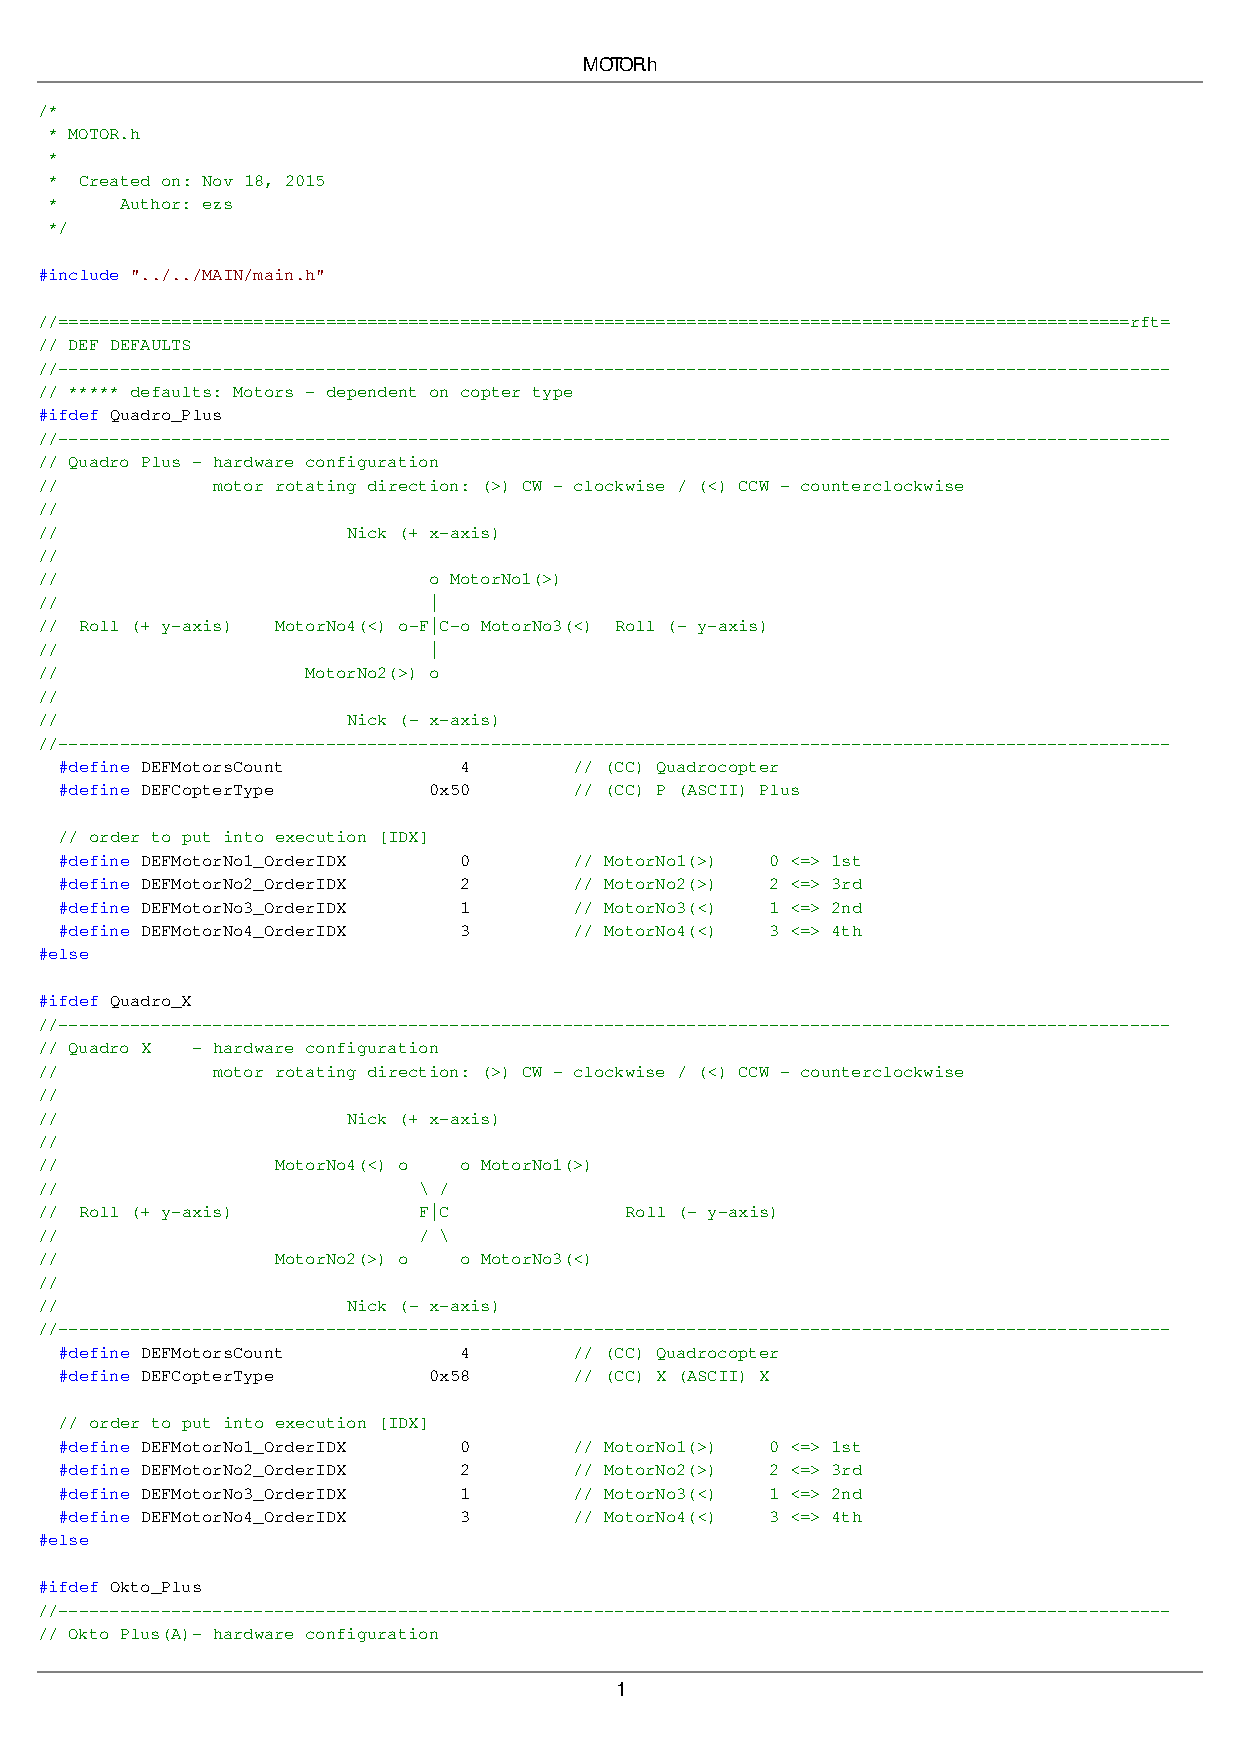
\includepdf[pages={1,2,3}]{fig_motor/pdf/MotorH.pdf}

\section{Script \textit{'testcase'}}
\label{script_testcase}
\begin{lstlisting}[language=bash]
#!/bin/bash
#Sets or Clear Flag to Run a testcase
#Used Parameter:
#	$1 - Testcase name which to set or clear
#	$2 - Optional Parameter set or clear the Testcase,if Unknown testcase will be set

#Path of file where all testacses are stored:
path="/home/pi/testfiles/_Testcases" 

if [ "$1" == '' ]
then
echo "First Paremeter does not exist, expected name of a testcase"
exit 1
else 
testcase=$1
fi

if [ "$2" == "clear" -o "$2" == "set" ]
then
if [ "$2" == "clear" ] 
then
mode=0
else
mode=1
fi
echo "mode $2 is used" 
else
mode=1
echo "used default mode set"
fi

if [ -e $path ]
then
echo "$path found"
else
echo "$path not found"
exit 2
fi

sed -i "s/^$testcase=[01]/$testcase=$mode/" $path
if [ $? == 0 ]
then echo "Command executed"
fi
\end{lstlisting}
